\documentclass[varwidth=true, border=2pt]{standalone}

\usepackage{pgfplots}
\usepackage{tikz}

\begin{document}
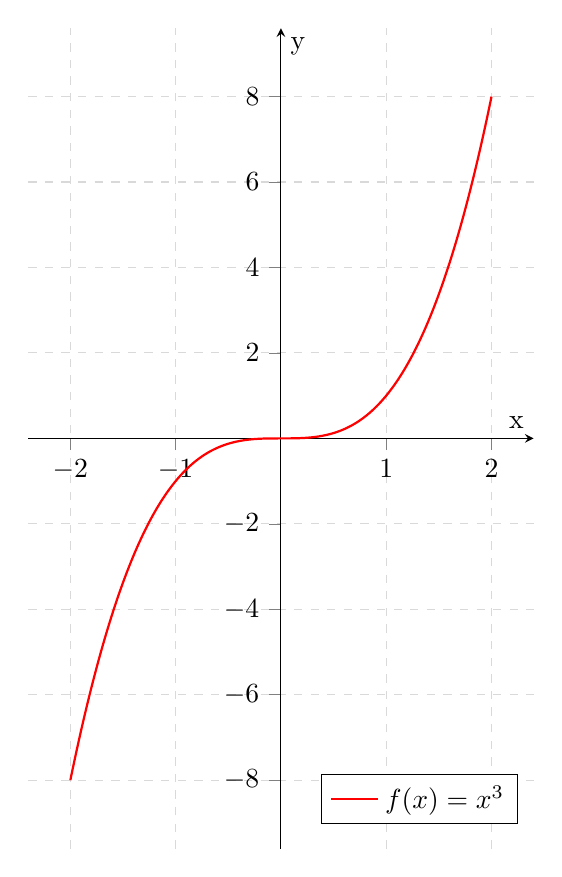
\begin{tikzpicture}
    \begin{axis}[
    legend pos=south east,
        axis x line=middle,
        axis y line=middle,
        grid = major,
        width=8cm,
        height=12cm,
        grid style={dashed, gray!30},
        xmin=-2,     % start the diagram at this x-coordinate
        xmax= 2,    % end   the diagram at this x-coordinate
        ymin=-8,     % start the diagram at this y-coordinate
        ymax= 8,   % end   the diagram at this y-coordinate
        axis background/.style={fill=white},
        xlabel=x,
        ylabel=y,
        %xticklabels={-2,-1.6,...,2},
        %yticklabels={-8,-7,...,8},
        tick align=outside,
        enlargelimits=true,
        tension=0.08]
      % plot the stirling-formulae
      \addplot[domain=-2:2, red, thick,samples=500] {x*x*x};
      \addlegendentry{$f(x)=x^3$}
    \end{axis}
\end{tikzpicture}
\end{document}
